\chapter{Introducción} \label{ch:intro}
\pagenumbering{arabic}

\section{Motivación}

La inteligencia artificial (IA) gana cada año más popularidad, impulsada por los últimos avances en tecnología y su aplicación en diversas industrias. La Figura \ref{fig:ai_grow} muestra el porcentaje de empresas que muestran interés en la IA y en la Figura \ref{fig:ai_market_size} se representa el crecimiento del valor del mercado de la IA en miles de millones de dólares.

\begin{figure}[htb]
  \floatsetup{heightadjust=all, valign=c}
  \begin{subcaptiongroup}
  \begin{floatrow}
	\ffigbox{%
  	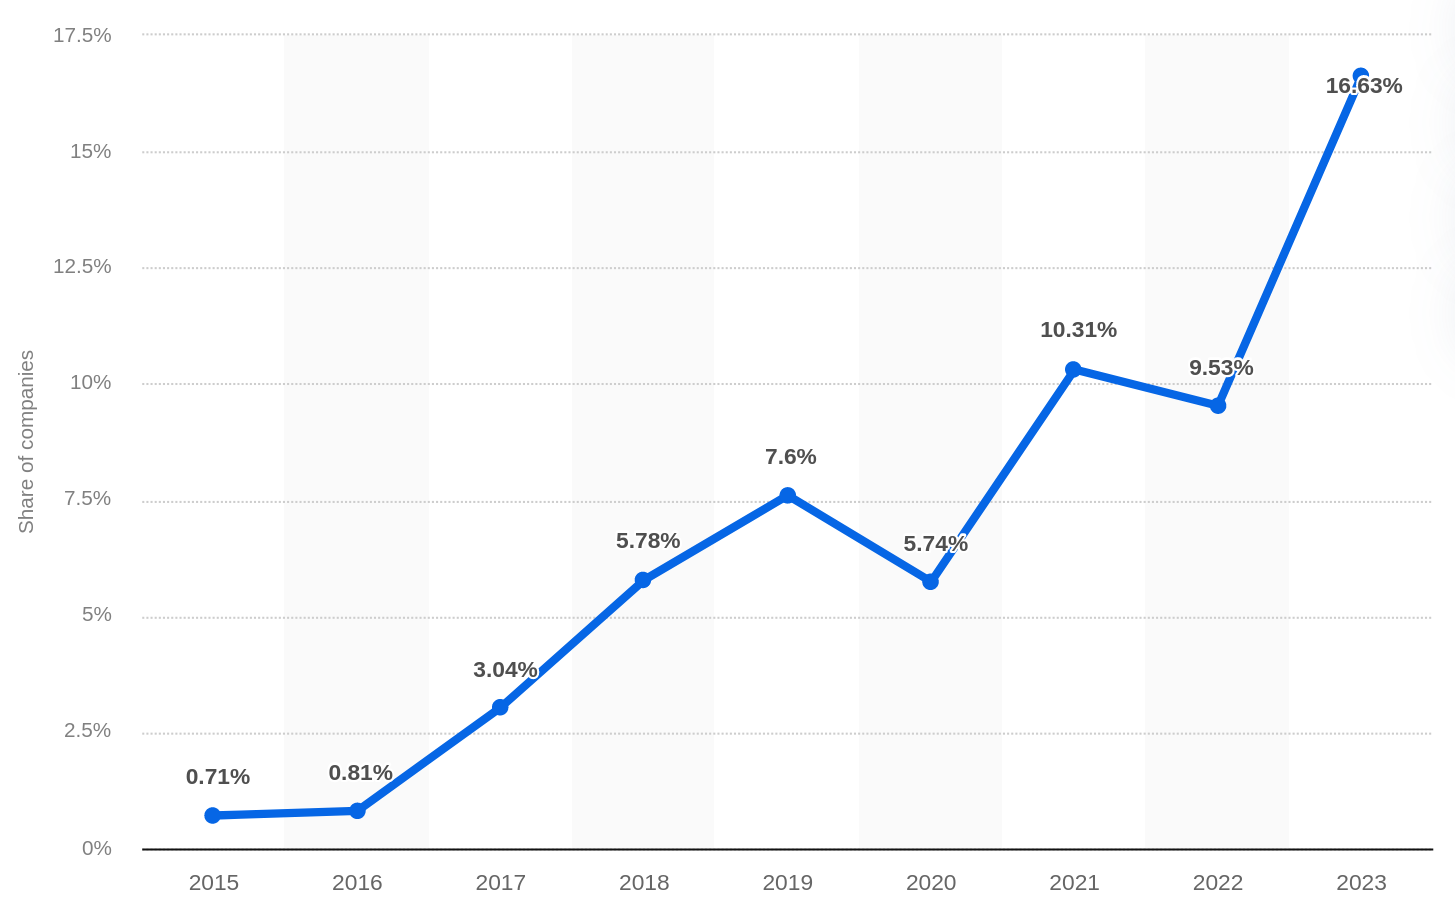
\includegraphics[width=0.48\textwidth]{root/Imagenes/intro/ai_interest.png}
	}{%
  	\caption{Interés de las empresas, representado mediante el porcentaje de empresas \cite{ai_interest_growth}.}
  	\label{fig:ai_grow}
	}
	\ffigbox{%
  	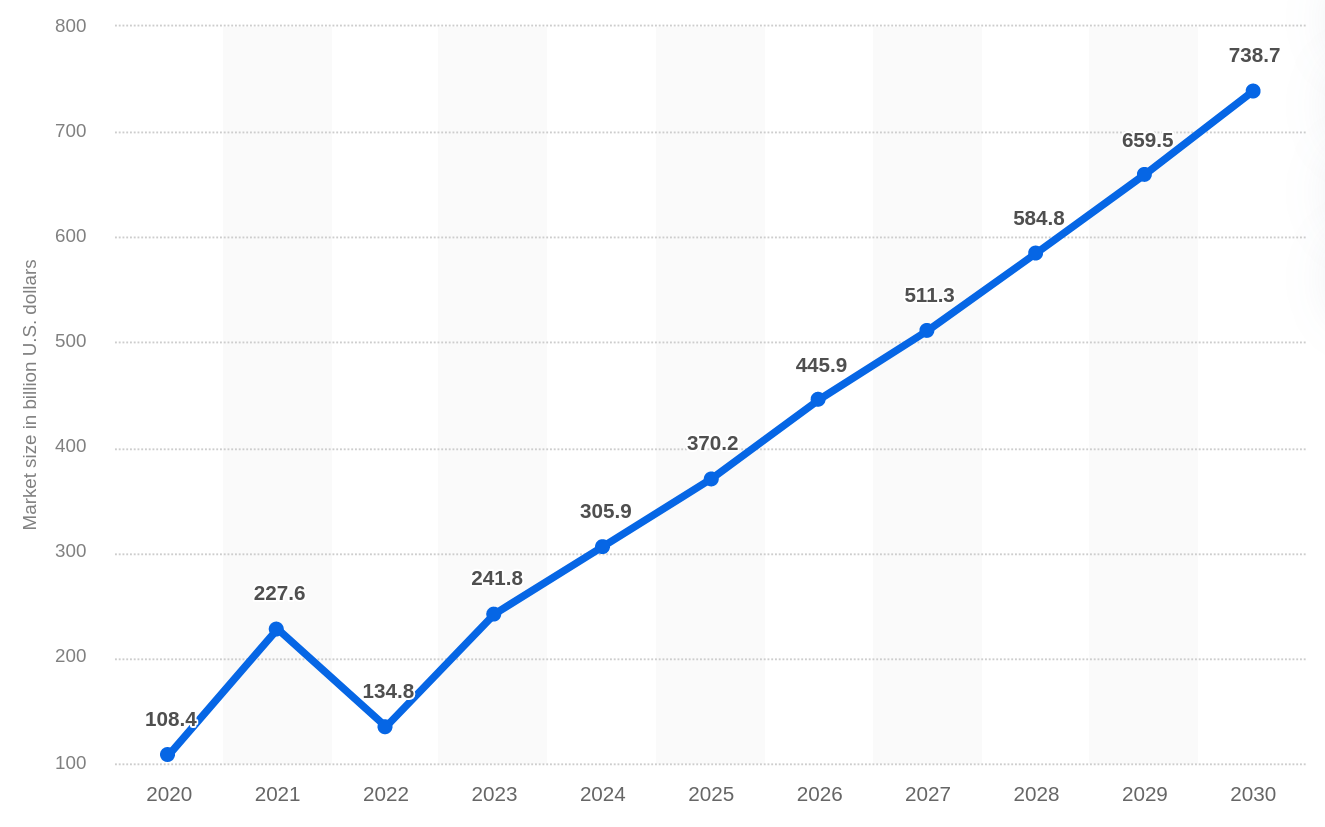
\includegraphics[width=0.49\textwidth]{root/Imagenes/intro/market_size.png}
	}{%
  	\caption{Valor de mercado en miles de millones de dólares \cite{ai_market_size}.}
  	\label{fig:ai_market_size}
	}
  \end{floatrow}
  \end{subcaptiongroup}
  \caption{Crecimiento de la IA en los últimos 10 años y crecimiento esperado hasta 2030.}%
\end{figure}

Al aumentar este interés y por tanto su uso en diversos campos también lo hará el consumo energético. La motivación principal de este trabajo es desarrollar componentes hardware para aumentar la eficiencia energética de la inferencia en un subconjunto de técnicas de aprendizaje automático. Concretamente, este trabajo se centra en las redes neuronales bayesianas (\textit{\textbf{B}ayesian \textbf{N}eural \textbf{N}etwork}). Estas redes calculan la incertidumbre de sus predicciones aportando transparencia en su uso. En relación, otra de las motivaciones de este trabajo es facilitar la adopción de estas redes para ayudar hacia el objetivo de la Unión Europea de trabajar con IAs más transparentes \cite{eu_ai}. Otra de las motivaciones principales de este trabajo es fomentar el desarrollo de la arquitectura RISC-V, que es una arquitectura de procesadores abierta y libre. Europa ha apostado por esta arquitectura, mediante el proyecto el \textit{European Processor Initiative} (EPI) \cite{european_processor}, para que sus empresas puedan diseñar y producir sus propios procesadores sin las restricciones y costos asociados con las arquitecturas propietarias tradicionales. 

Específicamente, este TFM aborda la ejecución de la inferencia de BNNs en dispositivos de bajas prestaciones orientados hacia la internet de las cosas (\textit{\textbf{I}nternet \textbf{o}f \textbf{T}hings}). Esta combinación se conoce comúnmente como TinyML y tiene un gran potencial a la hora de reducir el consumo energético \cite{tinyML_sustainable}. Los componentes IoT son más eficientes energéticamente que los procesadores de altas prestaciones, por lo que trasladar la ejecución de la inferencia de BNN a estos componentes reduciría su consumo además de eliminar comunicaciones costosas entre componentes IoT desplegados y servidores.

\section{Objetivos y alcance}

El objetivo principal de este trabajo es optimizar la inferencia de BNN en un procesador RISC-V de bajas prestaciones. Se han seguido los siguientes pasos para lograr el objetivo:
\begin{enumerate}
	\item Estudiar el funcionamiento de la inferencia de las BNN.
	\item Analizar aceleradores existentes de inferencia de BNN.
	\item Investigar el soporte existente para ejecutar inferencia de BNN en procesadores de bajas prestaciones sin precisión de punto flotante.
	\item Implementar una biblioteca en C junto a herramientas que permitan ejecutar la inferencia de BNN en un procesador RISC-V desarrollado en un trabajo previo \cite{riscv_tfg}.
	\item Validar la biblioteca implementada con diferentes modelos.
	\item Analizar la carga de trabajo de la biblioteca desarrollada.
	\item Desarrollar optimizaciones software y analizar sus ventajas y desventajas.
	\item Investigar sobre generadores de números aleatorios gaussianos (\textit{\textbf{G}aussian \textbf{R}andom \textbf{N}umber \textbf{G}enerator}).
	\item Diseñar un GRNG que se pueda integrar en el procesador RISC-V como una extensión.
	\item Estudiar los pasos necesarios para extender un procesador RISC-V y poder utilizar la extensión desde código en alto nivel C.
	\item Analizar el coste y rendimiento de la extensión utilizando una \textit{Field Programmable Gate Array} (FPGA).
\end{enumerate}

Todo el código de este trabajo se encuentra disponible en un repositorio público en GitHub \cite{bnn_github}.

%% quizas aqui se puede poner que lo hemos enviado al congreso y las JJI

\section{Estructura del documento}

El Capítulo \ref{ch:estado_arte} describe el estado del arte relacionado con la arquitectura RISC-V y las BNN. El Capítulo \ref{ch:metodologia} describe la metodología que se ha seguido durante el desarrollo del trabajo y las herramientas y modelos utilizados. En este capítulo también se explica la configuración experimental utilizada y los componentes que se han desarrollado para crearla. El Capítulo \ref{ch:motor_inferencia} explica las decisiones de diseño y desarrollo de una biblioteca para ejecutar inferencia de BNN en plataformas RISC-V y muestra resultados obtenidos con la misma. El Capítulo \ref{ch:optimizaciones} expone dos optimizaciones software para la inferencia de BNN implementadas en la biblioteca mencionada previamente. El Capítulo \ref{ch:extension} explica como se ha implementado una extensión para la inferencia de BNN en un procesador RISC-V y los resultados que se han obtenido con ella así como su eficiencia energética. Por último el Capítulo \ref{ch:conclusion} contiene las conclusiones y posible trabajo futuro.
